\pdfoutput=1
\documentclass[11pt]{article}
\usepackage[final]{acl}
% --- STANDARD PACKAGES REPLACING ACL.STY ---
% \usepackage[margin=1in]{geometry} % Standard margins
\usepackage{natbib}               % For citations
\usepackage{times}                % Times New Roman font
\usepackage{latexsym}
\usepackage[T1]{fontenc}
\usepackage[utf8]{inputenc}
\usepackage{microtype}
\usepackage{booktabs}
\usepackage{graphicx}
\usepackage{hyperref}             % Hyperlinks


% Define the \todo command if it was used in the template
\newcommand{\todo}[1]{\textcolor{orange}{[TODO: #1]}}

% --- TITLE AND AUTHORS ---
\title{Safety-Preserving Compression Between Generator and Safety Critic: \\ Measuring and Minimizing Safety Loss in Prompt-based PRM}

\author{
  Aidan Pinero \\
  UC Santa Cruz \\
  \texttt{apinero@ucsc.edu} \And
  Glenn Grant-Richards \\
  UC Santa Cruz \\
  \texttt{ggrantri@ucsc.edu} \And
  Sophia Yang \\
  UC Santa Cruz \\
  \texttt{syang255@ucsc.edu} 
}
\date{}

\begin{document}
\maketitle

\section{Paper Summary}

\begin{table}[h]
    \centering
    \small
    \begin{tabular}{lp{6cm}}
        \toprule
        \textbf{Title} & LLMLingua: Compressing Prompts for Accelerated Inference of Large Language Models \\
        \textbf{Venue} & EMNLP \\
        \textbf{Year}  & 2023 \\
        \textbf{URL}   & \href{https://arxiv.org/abs/2310.05736}{https://arxiv.org/abs/2310.05736} \\ 
        \bottomrule
    \end{tabular}
    \caption{Bibliographical information for the base paper.}
\end{table}

\noindent\textbf{Background} Large Language Models (LLMs) are increasingly applied in a wide range of domains. As language models become more powerful, the prompts they operate on tend to grow longer and more complex. However, lengthy prompts require substantial computational resources and increase inference cost. To address this, Jiang et al. (2023) proposed LLMLingua, a coarse-to-fine prompt compression method that maintains semantic integrity even at high compression ratios.

% \todo{Establish the scope for the paper focusing on LLM Agents.}



% Large Language Models (LLMs) are increasingly applied in a wide range of domains. As language models become more powerful, the prompts they operate on tend to grow longer and more complex. However, existing work has identified several challenges for LLMs in long-context settings. These challenges include higher computational costs, the presence of irrelevant or redundant information that hampers model performance, and position bias that causes LLMs to become “lost in the middle” (Jiang et al., 2023).

% The long-context issue is even more pronounced in LLM-based agents. Agent prompts often include role descriptions, instructions, and full trajectories that comprise chains of thought, tool calls and tool outputs, environment observations, and iterative revisions. In multi-agent systems, each round of communication further extends the shared context, quickly approaching the context-window limit.

% Current work has explored different approaches to compress prompts at roughly four levels of granularity: token level, token-/lexical-unit level, sentence level, and whole-passage level. These methods have made progress in improving efficiency and maintaining task accuracy under compression. However, they generally do not assess the loss of safety information during compression, even though safety preservation is a critical component of AI safety. In addition, to the best of our knowledge, there is little to no research that explicitly studies compression for agent prompts, particularly in multi-agent settings.

% To address these issues, we propose a safety-preserving compression framework for generator–critic agents, focusing on prompt-based process-level reward models (PRMs). Specifically, we introduce an intermediate compressor between a generator agent and a safety critic: instead of feeding the critic the whole, raw trajectory, we compress the generator’s prompt and internal trace while explicitly measuring and minimizing the resulting safety loss - the degradation in the critic’s ability to detect or prefer safe behavior. This design allows us to (i) retain most of the efficiency benefits of prompt compression, (ii) quantify how much safety signal is lost at different compression levels, and (iii) optimize the compressor to preserve safety-relevant information, rather than treating safety as an implicit side effect. \newline


\noindent\textbf{Summary of contributions} They introduce LLMLingua, which lays the foundation for subsequent compression methods. Their approach consists of a budget controller, iterative token-level compression, and an alignment module. They validate the effectiveness of their method, achieve state-of-the-art performance, and significantly reduce computational resources, demonstrating clear practical value.
% \todo{Summarize the contributions made by this work.}



% The contribution of our work is threefold. First, we introduce compression explicitly into the agent setting, designing compressors that account for agent-style trajectories rather than generic text. Second, we focus on small language agents that are suitable for future on-device deployment; such agents naturally have limited computational resources and context windows, making compression especially important. Third, we evaluate the often-ignored safety loss under compression and aim to make compression more safety-preserving, rather than optimizing solely for efficiency and accuracy.

\paragraph{Limitations and discussion}LLMLingua is a token-level approach for compression. Token-level pruning is computationally efficient, but it can easily produce fragmented or ungrammatical text (Zhao et al., 2025). This harms human interpretability, and the loss of safety-relevant information may raise additional risk.

In addition, this work focuses on efficiency and does not assess the loss of safety information during compression, even though safety preservation is a critical component of AI safety. Compared to our proposed research, it targets language-model prompts and is not designed for agent prompts that include role descriptions, instructions, and full trajectories comprising chains of thought, tool calls and tool outputs, and environment observations, and is even less applicable to multi-agent settings.
% \todo{Discuss the limitations.}



\paragraph{Why this paper?} We chose Jiang et al. (2023, LLMLingua) as our primary paper to analyze because it is one of the earliest and most influential works on prompt compression and has inspired many subsequent studies. It proposes a token-level, coarse-to-fine compression framework for black-box LLMs, directly relevant to our safety setting: in many harmful or unsafe cases, one or two critical tokens can determine whether a behavior is safe. Understanding how LLMLingua allocates budgets and prunes tokens under high compression, therefore, provides a natural starting point for designing and evaluating safety-preserving compression between a generator and a safety critic.
% \todo{Discuss the motivation for choosing this paper.}


\paragraph{Wider Research Context}

\section{Project Description}
\subsection{Generator-Safety Critic Framework}

The Generator-Safety Critic framework is a dual-agent architecture designed to decouple task performance from safety compliance. In this pipeline, the Generator (typically an instruction-tuned SLM or LLM) focuses purely on satisfying user intent, often producing verbose "process traces" or reasoning steps (Chain-of-Thought) to improve performance. The Safety Critic acts as an independent auditor, evaluating the Generator’s output against a specific safety constitution or policy before it reaches the user. This separation is critical because it allows the Generator to remain helpful and creative without being overly inhibited during generation, while the Critic ensures final alignment. For on-device applications with scarce computational resources, this framework allows developers to use a smaller, less robust Generator, relying on a specialized Critic to catch failures or “jailbreaks” that the smaller model might miss.

The industry standard for this "Critic" role currently relies on specialized guard models and rule-based frameworks. Prominent examples include Meta’s Llama Guard 3 (and the 3.1 Nemotron variant), NVIDIA’s NeMo Guardrails, and Azure AI Content Safety. These models are fine-tuned classifiers trained to detect specific categories of harm (e.g., PII, hate speech, self-harm) and output a binary "safe/unsafe" decision or a risk score. Frameworks like Constitutional AI (pioneered by Anthropic) further refine this by asking the Critic to evaluate and revise content based on natural language principles rather than relying solely on labeled data.

Despite their utility, current guard models face a critical bottleneck: contextual inefficiency. Safety Critics often struggle with the "Refusal-Helpfulness" trade-off: they either over-refuse benign queries because they lack the context to understand nuance, or they fail to detect subtle attacks (such as “Needle in a Haystack” injections) buried deep within long Generator outputs. Furthermore, for a Safety Critic to be effective, it needs to read the entire reasoning trace of a Generator. If the Generator produces a 4,000-token explanation, a standard on-device Safety Critic with a limited context window (or strict latency budget) cannot process it all.

This introduces the necessity of a Compressor. A Compressor agent acts as an intelligent intermediary, synthesizing the Generator’s verbose "evidence packet" (intent, key steps, warnings) into a dense, safety-salient summary. By filtering out irrelevant fluff while preserving "safety-relevant" signals, the Compressor allows a smaller, limited-context Safety Critic to make accurate judgments without the computational cost of processing raw, massive contexts. This essentially means "lossy compression for semantics but lossless for safety," which is the missing link for enabling robust safety checks on resource-constrained devices.

\subsection{The Generator-Compressor-Safety Critic Pipeline}

This project investigates a novel safety architecture for on-device Small Language Models (SLMs) that operate under strict compute and context constraints. The pipeline introduces a "Compressor" agent between the task-performing Generator and the Safety Critic (a prompt-based Process Reward Model). In this setup, the Generator produces a detailed, step-by-step response to a user query. Before this verbose "evidence packet" reaches the limited-context Safety Critic, the Compressor summarizes it, retaining all safety-relevant information (intents, warnings, tool calls) while discarding irrelevant tokens. The core research question is whether this compression degrades the Safety Critic's ability to detect harm. We measure this by comparing the Safety Loss—the discrepancy in risk detection between a baseline (Critic sees full text) and our method (Critic sees compressed text).

\subsection{Dataset Architecture: Attacks and Ground Truth}

To rigorously stress-test this pipeline, we utilize three benchmark datasets: AgentDojo, LLMail-Inject, and Lakera PINT. These datasets are structured around two distinct components: the Attack and the Ground Truth.
In our experimental design, we conceptualize the “Attack” not just as the input prompt, but as the realized unsafe behavior generated by the Generator. While the datasets provide malicious inputs (e.g., an incoming email with hidden instructions or a “jailbreak” prompt), the actual "attack" occurs when the Generator (the victim SLM) processes these inputs and produces a harmful response or executes a forbidden tool call. For example, in AgentDojo, the dataset feeds the Generator a tool output containing a hidden "ignore previous instructions" command. The "attack" is successful if the Generator executes the malicious command (e.g., exfiltrating data) instead of completing the user’s benign task.

The Ground Truth serves as the objective reference for calculating our primary metrics: Unsafe Pass-through Rate (Attack Success Rate), Attack Miss Rate, and Over-refusal Rate. For AgentDojo and LLMail-Inject, the ground truth is functional: did the Generator actually execute the specific forbidden tool call (e.g., `send\_email` to an attacker)? This allows us to definitively label the Generator’s output as "unsafe."

For Lakera PINT, the ground truth is a labeled classification (Safe/Unsafe) associated with the input prompt. By comparing the Safety Critic’s decision (Approve/Refuse) against this objective Ground Truth, we can determine if the Compressor successfully preserved the "evidence" of the attack. If the Generator produces an unsafe tool call (Ground Truth = Unsafe) but the Critic approves it after reading the compressed summary, we know the Compressor failed to preserve the safety signal, contributing to the “Attack Miss Rate."



\paragraph{Goal} 
The primary motivation for this project is the constraint on context windows in Generator-Safety Critic multi-agent pipelines. In such pipelines, the Critic's judgment depends on evidence received from the Generator, which can be very long. Reading the entire context is costly and limited by the Critic's context window.

Our goal is to introduce a compressor agent to solve this bottleneck. We aim to measure and minimize safety loss when summarization or truncation is applied.

\paragraph{Task}
The task involves a multi-agent pipeline consisting of a Generator, a Compressor, and a Safety Critic. 
\begin{enumerate}
    \item \textbf{Generator:} Produces a structured response with a public process trace (no hidden Chain-of-Thought).
    \item \textbf{Compressor:} Converts the Generator output into a shorter "evidence packet" for the Critic.
    \item \textbf{Safety Critic:} A prompt-based Process Reward Model (PRM) scores each step and output, producing a decision (APPROVE/REWRITE/REFUSE).
    \item \textbf{Loop:} If the decision is REWRITE, constraints are sent back to the Generator to revise.
\end{enumerate}

\begin{figure}[h]
    \centering
    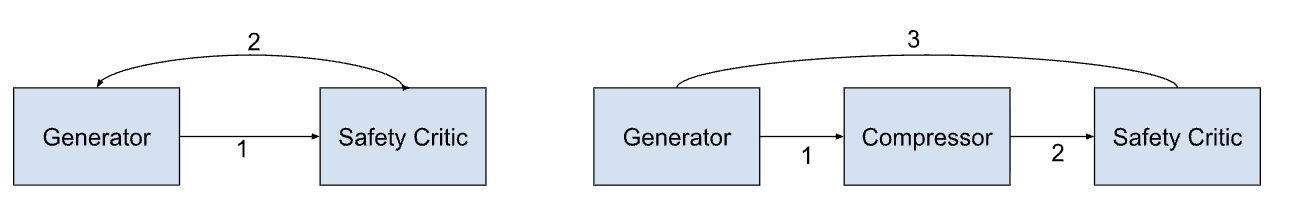
\includegraphics[width=1\linewidth]{Pipeline graph.png} 
    \caption*{Proposed Pipeline: \newline (1) Generator $\rightarrow$ (2) Compressor $\rightarrow$ (3) Safety Critic}
    \label{fig:pipeline}
\end{figure}

\paragraph{Data}
We will utilize the following datasets:
\begin{itemize}
    \item AgentDojo
    \item LLMail-Inject
    \item Lakera PINT Benchmark
\end{itemize}

\paragraph{Methods}
We propose a compressor agent situated between the Generator and the Critic.
\begin{itemize}
    \item \textbf{Architecture:} A sub-1 billion parameter model acting on chunked content to ensure cost savings.
    \item \textbf{Implementation:} We will investigate whether to use an encoder projecting into guards embedding space or a decoder-based approach.
    \item \textbf{Safety Critic:} We will use Llama-Guard-3-8B as the underlying model.
\end{itemize}

\paragraph{Baselines}
\begin{itemize}
    \item \textbf{Baseline:} Generator-Safety Critic framework with \textbf{no compression}.
    \item \textbf{Group 1 (Naive):} Critic sees a short summary or truncated text.
\end{itemize}

\paragraph{Evaluation}
We will measure:
\begin{itemize}
    \item \textbf{Unsafe Pass-through Rate:} Percentage of harmful prompts resulting in unsafe content.
    \item \textbf{Attack Miss Rate:} False negative rate.
    \item \textbf{Over-refusal Rate:} False positive rate.
    \item \textbf{Safety Metric Accuracy:} Checks if accuracy decreases with compression.
\end{itemize}

\subsection{Models}
\noindent \textbf{Generator: Baseline Agent} 

To isolate the effect of compression on safety, we require a baseline to compare to. We implement a "dummy" generator that strictly reproduces traces and responses directly from our evaluation dataset (AgentDojo). This creates a reproducible set of known "safe" and "unsafe" outputs we can compare our compressed model to and will serve as the input source for our pipeline. \newline

\noindent \textbf{Compressor: Perplexity-Based Evidence Extractor} 

Long context windows are computationally expensive and can suffer due to the "Lost in the Middle" phenomenon. We utilize a small, efficient proxy model to act as a compressor. It processes the generator's response, retain important information and discarding redundant context. This is the core variable of our study and we will measure how its compression ratio impacts downstream safety visibility. \newline

\noindent \textbf{Safety Critic: Llama Guard 3} 

We will use Llama Gaurd as an automated judge to verify output safety. It receives the compressed response (the "evidence packet") from the compressor and acts as the final decision-maker, classifying the interaction as safe or unsafe. This model serves as the constant baseline in our experiment, as we test its ability to maintain classification accuracy when its input context is severely truncated.

\subsection{Metrics}
\noindent \textbf{System Attack Success Rate (System ASR)} 

Standard ASR measures if a generator produces a harmful output; but we will measure if the critic misses that output. We define System ASR as the False Negative Rate: the probability that the critic outputs "Safe" given that the Generator produced known "Unsafe" content. We will use this as our primary failure metric. A rise in the ASR relative to the baseline will indicate that compression has lose information, allowing safety violations to pass through undetected. Contrarily, a decrease will show that the compressed model gains benefits in both cost and safety compared to the model. \newline

\noindent \textbf{Benign Refusal Rate (BRR)} 

A system could refuse all inputs and be secure but it would essentially be useless. Benign Refusal Rate measures the False Positive Rate: how often the critic flags safe, benign content as harmful. We will use this metric to evaluate the usability cost of compression. It allows us to detect if the compressor causes the critic to hallucinate safety violations where none exist.

\subsection{Experiment group setup}

\textbf{Control group} uses a standard generator–safety-critic architecture without any intermediate compression.

\noindent\textbf{Compression baseline} inserts a compressor agent that applies naive strategies such as simple truncation or fixed-length clipping before passing trajectories to the safety critic.

\noindent\textbf{Proposed group} follows a generator-compressor-safety-critic architecture, but the compressor is implemented as a small agent trained with more principled techniques

\subsection{Literature Review}
\subsubsection{Existing Generators}
\textbf{Small Language Models (SLMs) as Agentic Generators}

The Shift to Capable Small Language Models (SLMs) has challenged the assumption that agentic workflows require massive models, with a new wave of SLMs (typically <8B parameters) optimized for on-device inference and complex reasoning. Microsoft’s Phi-3 (specifically the 3.8B Mini and 14B Medium) is a primary candidate for the “Generator,” having demonstrated performance comparable to GPT-3.5 on reasoning benchmarks by utilizing high-quality “textbook-quality” training data. Similarly, Google’s Gemma 2 (2B and 9B) and Meta’s Llama 3.2 (1B and 3B) are explicitly designed for edge deployment, offering a balance of instruction-following capability and low latency that fits the constraint of a “limited context window” and cost-sensitive pipeline. These models are sufficiently capable of producing the “structured response” and “public process trace” required by our protocol while remaining small enough to justify a separate, compressed safety check. \newline

\noindent \textbf{Generators in Safety \& Injection Benchmarks} 

In the target datasets, the choice of Generator often dictates the baseline vulnerability. AgentDojo and Lakera PINT typically benchmark larger models (e.g., GPT-4o, Claude 3.5 Sonnet), which act as robust baselines; however, replacing these with SLMs introduces distinct safety dynamics. Research using the LLMail-Inject dataset has already begun to validate this shift, using Phi-3-medium as a target victim to test indirect prompt-injection defenses. This is particularly relevant as SLMs often exhibit higher “Attack Success Rates” (ASR) due to less robust safety alignment compared to their larger counterparts, making the role of Safety Critic and Compressor even more critical. Using an SLM as the Generator also aligns with the “weak-to-strong” generalization paradigm, where a specialized critic supervises a smaller, potentially unsafe generator. \newline

% \noindent \textbf{Reasoning Capabilities for Process Traces}

% For the Generator to produce a “public process trace” (Chain-of-Thought), it must possess strong multi-step reasoning capabilities despite its size. “Reasoning” models like DeepSeek-R1-Distill (Qwen/Llama variants) or Orca-2 have been fine-tuned specifically to output detailed explanatory traces, making them ideal Generators for a Process Reward Model (PRM) pipeline. Unlike standard completion models, these are trained to articulate intermediate steps, providing the raw “evidence” (intent and key steps) that the Compressor agent needs to summarize. Selecting a Generator with these specific fine-tuning characteristics will ensure that the evidence packet contains rich, audit-ready information for the Safety Critic to evaluate.




\subsubsection{Metrics}
\textbf{HarmBench: A Standardized Evaluation Framework for Automated Red Teaming and Robust Refusal}
Prior to HarmBench, measuring safety involved manual attacks or checking for refusals using string matching. HarmBench standardized safety evaluation, by using automated red-teaming and finding the ASR (attack success rate), which calculates the validity of a model's defense and uses a judge to classify if a response is actually harmful, rather than relying on the model's self-reported refusal. This paper provides the ground truth metric we will use. We will use its evaluation methodology to determine if our compressor caused the critic to miss an attack that a standard HarmBench evaluation would have caught. \newline

\noindent \textbf{Llama Guard: LLM-based Input-Output Safeguard for Human-AI Conversations}

Llama Guard is an ideal language model for classifying the safety of a model, since it is open-weights and fine-tuned specifically for safety classification. It analyzes the semantic relationship between a user's input and an agent's output against a set of rules, judging between safe and unsafe responses. This is the architecture we will use for our critic and will be the baseline we will compare to.



\subsubsection{Compression Techniques}

Existing studies approach prompt and context compression at roughly four granularity levels in terms of what is being compressed: tokens, lexical groups, sentences, and the entire prompt representation. \newline

\noindent\textbf{Token-level methods} 

This line of work treats individual tokens as the basic unit of selection or deletion. There are machine-learning–based approaches. For example, Pan et al. (2024) proposed LLMLingua-2, which explicitly formulates compression as a token-level binary classification task. A small compressor model predicts keep/drop labels for each token and removes those predicted as unimportant. They preserve the faithfulness of the compressed prompt by constraining the compressor model from generating new tokens. There are also attention–mechanism–based approaches. For example, Fei et al. (2025) proposed Evaluator Head-based Prompt Compression (EHPC). In this work, they identify a small set of “evaluator heads” - attention heads that can be used to quickly determine the necessity of a token - and use their attention weights during the pre-filling stage to score and retain only high-utility tokens. 

% Token-level pruning is computationally efficient, but it can easily produce fragmented or ungrammatical text (Zhao et al., 2025). This harms human interpretability, and the loss of safety-relevant information may raise additional risk concerns. \newline

\noindent\textbf{Lexical-group-level methods.} 

Zhao et al. (2025) argue that token-level approaches evaluate each token independently, ignoring phrase-level cohesion, and that aggressive token deletion often results in non-coherent sentences. To mitigate this, they introduce AttnComp, hypothesizing that attention values reflect the degree of semantic dependency and leveraging attention patterns to group tokens into semantic units via a graph-based algorithm. Their algorithm minimizes cross-group dependencies: tokens are first clustered into coherent lexical groups, and compression is then applied at the group level, yielding more cohesive spans that better preserve sentence-level meaning and downstream performance. \newline

\noindent\textbf{Sentence-level methods.} 

Similarly motivated by the limitations of token-level approaches, Liskavets et al. (2025) propose Context-aware Prompt Compression (CPC), which operates at the sentence level. CPC aims to compress long prompts by removing sentences that are less relevant to the question while preserving human readability. Their study trains a context-aware sentence encoder with a contrastive objective to distinguish sentences that contain information relevant to the answer from those that do not. Sentences are ranked by their relevance to the query using embedding similarity, and the compressor then drops low-ranked sentences, producing shorter but still grammatical prompts that avoid the non-coherence and semantic drift observed in token-based methods under high compression. \newline

\noindent\textbf{Whole-prompt-level methods.} 

Another line of work compresses prompts at the whole-prompt level. One direction is embedding-style compression. For example, In-Context Autoencoder (ICAE) learns a LoRA-adapted encoder on top of the target LLM to map a long context into a small number of continuous “memory slots,” which then replace the original tokens in the decoder’s context window. Another direction is textual paraphrase–style compression, such as Nano-Capsulator, which uses another LLM to paraphrase the original prompt into a shorter natural-language prompt while attempting to preserve its essential semantics.

% Across these granularities, training and optimization strategies typically fall into three families summarized by the empirical study on prompt compression: (i) RL-based methods, which learn to select text spans using heuristic rewards without ground-truth compressed labels; (ii) LLM-scoring methods, such as LongLLMLingua, which use an auxiliary LLM to assign importance scores to tokens and make keep/drop decisions in a single autoregressive pass; and (iii) LLM-annotation methods, such as LLMLingua-2, which use a strong LLM to annotate compression labels and then train a smaller dedicated compressor model.

Despite substantial progress on efficiency and task-level accuracy, these techniques have several limitations for safety-centric, multi-agent settings. First, they are almost entirely designed for single-model, text-only prompts, with little attention to compressing tool-calling traces or multi-agent dialogue states. Second, existing evaluations and objective functions are dominated by utility metrics and largely ignore safety loss. This leaves open space for compressors that (a) operate over richer agent traces (including tool calls) and (b) explicitly trade off efficiency, task utility, and safety preservation, which is the niche our generator-compressor-safety-critic pipeline aims to target.




\bibliography{references} 
\nocite{*}
\end{document}
